\section{Motivation}

The most important energy conversion devices nowadays are electric machines which includes motors and generators. They are used with different specifications, structures and ratings in various applications, such as aerospace \parencite{bouzidi2015electromagnetic}, transportation \parencite{bilgin2019modeling}, power generation \parencite{saruwatari2016design} and healthcare \parencite{nicolaescu2012rotary}. Depending on the application, different optimal performance parameters, such as efficiency \parencite{mccoy2014premium}, noise and vibration \parencite{wang2016neural}, \parencite{sheikman2014methods} and torque ripple \parencite{baek2014optimal}, might be required.
This makes electromagnetic analysis and optimization the basic ingredients for the development of an electric machine. 
The designing of an electric motor is generally a rigorous, highly knowledge- or experienced-based, and time-consuming procedure \parencite{mayr2018electric}. During the product development procedure, from design and optimization through to manufacturing and test stages, a common flow of product development is followed, which is also known as V-design cycle (VDC) \parencite{sharafi2013knowledge, rivera2017knowledge}. This product development process of electric motors consists of two main stages, namely design and manufacturing. The overview of the proposed automated design and manufacturing process for electric motor drives is illustrated in Figure \ref{fig:INTRO_The_V_Design_and_Manufacturing_Cycle}, along with the principal components.

\begin{figure}[h!]
    \centering
    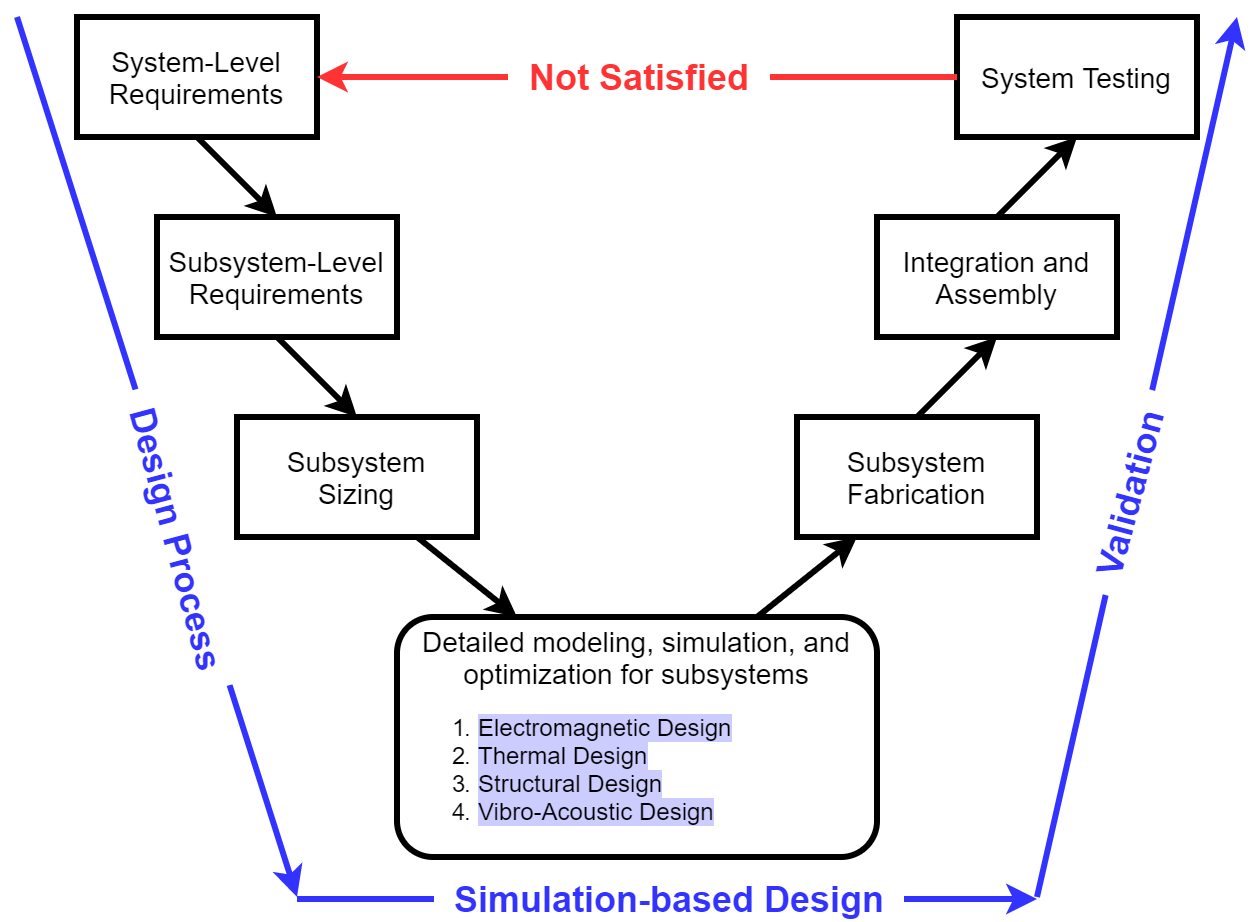
\includegraphics[width=\textwidth]{Figures/Chp_Intro/Intro2.png}
    \caption{The V-Design and Manufacturing Cycle}
    \label{fig:INTRO_The_V_Design_and_Manufacturing_Cycle}
\end{figure}

Given a machine's specification, the goal is to find a winning candidate in terms of performance and to make sure the candidate satisfies all the design criteria.
The `Design Phase' in the V-Design cycle is a critical stage since the product requirements, i.e. system- and subsystem-level, are specified in this stage to perform a simulation-based engineering design and optimization of the subsystems (motor, inverter, gearbox, battery, and charger, etc), that are then passed to the next stage in order to make sure the implemented system satisfies the initial specifications \parencite{ghorbanian2017computer}. 
There can be a significantly high number of possible candidates in a design space for a machine, even after applying the design and engineering constraints.
Since sophisticated simulation and design optimization tools, i.e. (FE) packages, are used to analyze the multiphysics performances, the wall-clock time for finding an optimal design directly depends on how fast the simulation and optimization processes are \parencite{tuchsen2018data, silva2018surrogate}. The required resources, including time, money, and high-performance computing services, will increase dramatically if the process is to be repeated for all new designs or applications. In such a scenario, it is infeasible to rank all the possibilities before choosing an optimal solution due to the massive computational burden involved in the analysis through conventional techniques. Hence, only a handful of potential designs obtained through the design cycle undergo a full multi-physics simulation at any stage in the design process. Finally, a prototype is manufactured and its performance is experimentally verified. 

In case the design or prototype does not meet the desired requirements, the process has to restart. This cycle can be reduced if the design space can be searched based on a multi-physics solution. However modern computer tools for analysis (at high fidelity), will take too long as there are hundreds or even thousands of design candidates. Hence, a need to formulate alternative strategies to ease the computational cost involved in the process. This has the potential to reduce the research cycle associated with product development. 
This thesis will look at some novel ideas for the design and analysis of electric devices and machines, ranging from surrogate models for fields and performance maps to intelligent agents for design optimization.
All the data-driven methodologies discussed in this work originate from the field of statistical learning.  

\begin{comment}

\begin{figure}
    \centering
    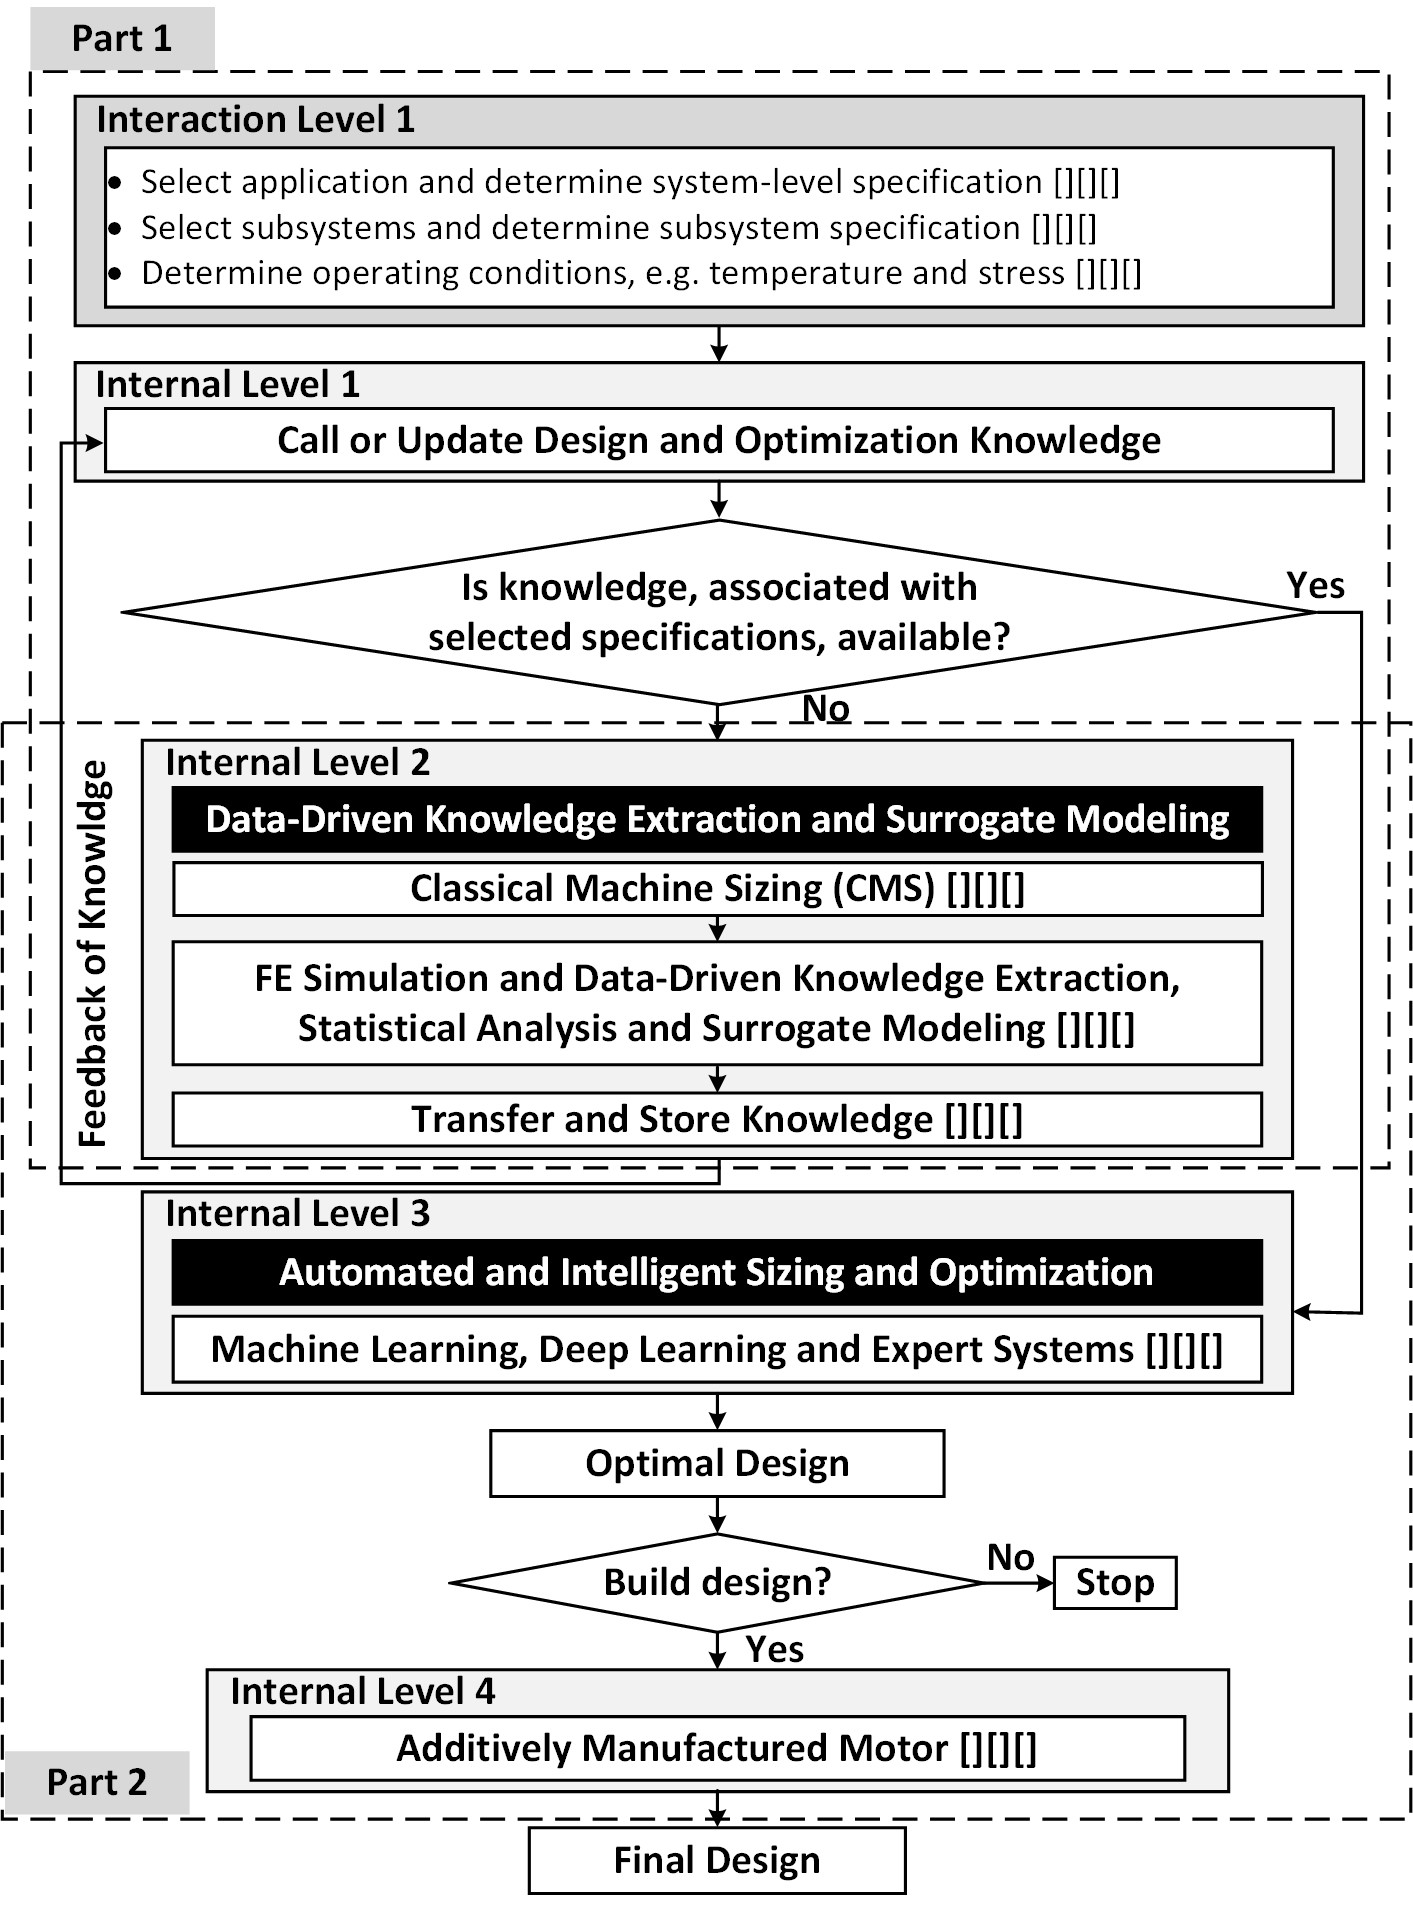
\includegraphics{Figures/Chp_AM/Automated_design_and_manufacturing_process.jpg}
    \caption{Automated design and manufacturing process}
    \label{fig:INTRO_Automated_design_and_manufacturing_process}
\end{figure}

\begin{figure}[h!]
    \centering
    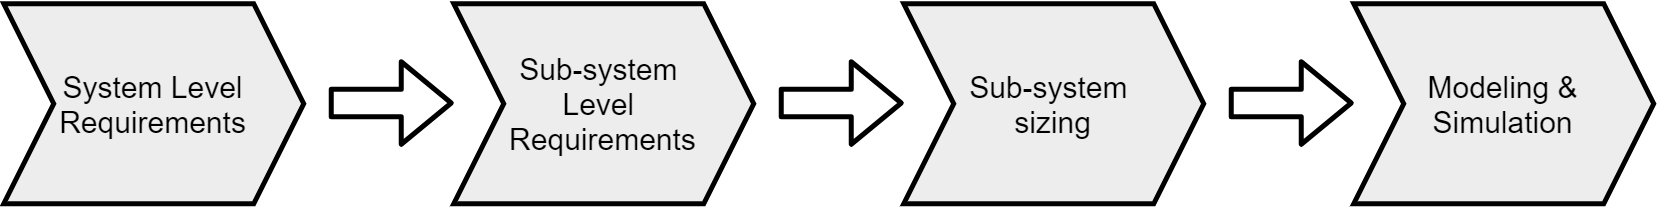
\includegraphics[width=\textwidth]{Figures/Chp_Intro/Flattened_V_cycle.png}
    \caption{Flattened V-cycle}
    \label{fig:INTRO_Flattened_V_cycle}
\end{figure}

\begin{figure}
    \centering
    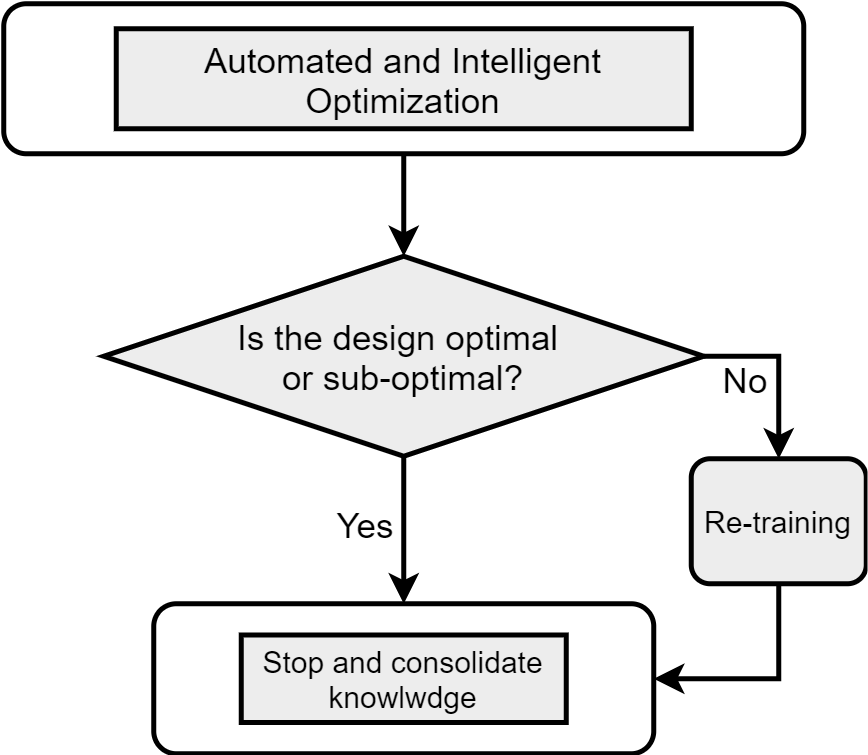
\includegraphics[width=0.5\textwidth]{Figures/Chp_Intro/Plan_for_intelligent_agent.png}
    \caption{Plan for intelligent agent}
    \label{fig:INTRO_Plan_for_intelligent_agent}
\end{figure}

(1) Specs for the desired EM device are developed from a design of the complete system 

Ex. For an electric vehicle, specification for the motor developed from the drive cycle of the device 

(2) Potential designs are considered and an optimization process is carried out. One or a few candidate solutions are chosen 

(3) Simulate: A 2D and 3D physics solution is created for each candidate 

(4) Optimization step across this now limited set of solution 

(5) Finally a full multi-physics simulation is implemented 

Thermal, structural, NVH, EMI, EMC 

(6) A prototype is constructed and verification of its performance is carried out 
\end{comment}

Machine Learning (ML) algorithms, specifically feedforward neural networks (FNN) have been shown as suitable candidates for function approximation. The application of this has been seen in the usage of neural networks as surrogates for performance evaluation metrics (such as Torque) have become prominent in the past couple of decades \parencite{ghorbanian2018hpc, wlas2008neural}. Alternatively, electrical machines can also be designed using an equivalent circuit (or lumped parameter approach). These methods can provide a fast prediction of global performance parameters such as average and ripple torque. 
However, these models cannot produce information on local effects within the device such as fields, losses, and stresses. 
Due to these complexities and limitations, big data, Artificial Intelligence (AI), Machine Learning (ML), and data mining tools seem to be promising ways to keep up with the ever-increasing demand of fast and accurate analysis of electric designs \parencite{kisskalt2018towards, khan2020efficiency, salimi2018computer, ghorbanian2019hpc}.  This work focuses on technologies that broadly include (a) modern machine learning techniques, such as deep learning carried out with the aid of high-performance computing, and (b) intelligent generative design, such as the topology optimization for flexible and complex shape design.

\section{Overview of Thesis Contribution}

The thesis is organized into six chapters and in terms of the research methodology of AI, the work performed here can be broadly classified into two categories: supervised learning and reinforcement learning. However, the algorithms have been extended as per the requirement of the task being considered. As an example, the supervised learning task in Chapter \ref{chapter:2_CNN} was extended to incorporate Bayesian learning to develop an indication of algorithm confidence in the prediction. Similarly, the usage of certain algorithms such as the attention mechanism was modified (as compared to \parencite{bahdanau2014neural}) to better suit the task of efficiency prediction in Chapter \ref{chapter:3_RNN}. 

\newpage

This section presents an overview of all the chapters of this thesis, along with the author's contribution.

\subsection{Application of Deep Learning for Electric Machine Performance Analysis}

For designing surrogates for the global quantities, (e.g. the torque ripple) which have a limited number of output values, usually one, for each motor design, the task is simple enough to be handled by a simple feedforward neural network. However, fully connected neural networks usually lose their attractions when it comes to many input-many output design and modeling problems, due to the required training complexity, while the same problem can be handled more efficiently using the deep Convolutional Neural Networks (CNNs) and/or Recurrent Neural Networks (RNNs). One example of such kinds of problems is modeling a local quantity of an electric motor, such as the magnetic flux density, where hundreds or thousands of numerical values distributed on the mesh structure of an FE solution should be predicted. 

Chapter \ref{chapter:2_CNN} deals with the problems of many electric devices operating at electrical power frequency (50Hz).  
The advantages and limitations of such methods for a variety of problems are also discussed. In addition to task compatibility, the change helped improve the speed of training \parencite{khan2019deep}.

The author is responsible for handling the data generation along with development and validation of all DL models associated with the study. The findings of this Chapter are presented in \cite{khan2019deep}, with other authors contributing with guidance on the research methodology, reviewing of manuscript and analysis of the results.

\subsection{Surrogate Model for Performance Maps}

Extending the usage of deep networks such as CNN, and RNN, is used for predicting performance parameters of electric motor drives \parencite{khan2020efficiency}. The RNNs are useful when a variable number of inputs, outputs, or both exist. The efficiency, power factor, losses, and advance angle maps of an electric motor drive are clear examples of this application.
Further, the usage and application of such networks are extended to predict higher dimensional output spaces such as performance maps, which will be discussed in Chapter \ref{chapter:3_RNN}. The prediction time of performance maps is reduced considerably to a few seconds for multiple geometries, against hours required for traditional approaches \parencite{mohammadi2017computational}.

Two papers (\cite{khan2020efficiency} \& \cite{khan_transfer}) were published based on the results obtained in Chapter \ref{chapter:3_RNN}. The author is partially responsible for handling the data generation and solely performed the analysis and validation of components associated with DL models, along with formulating the experiment associated with transfer learning (Section \ref{RNN:7_TL_methodology}). Other authors involved in this work contributed in conception of the research work, acquisition of data, interpretation of results and drafting of the article.

\subsection{Topology Optimization}

The most noticeable advantage of the Topology Optimization (TO) is its capability of free-shape optimization, which can outperform template-based design optimization routines in terms of the speed of the process if well-tuned. 
However, the majority of the TO techniques introduced in the literature result in solutions that are not easily manufacturable, i.e., the optimized design has checkerboard patterns, floating or stray pieces of material.
To overcome this difficulty, either different filtering or smoothing methods are employed \parencite{campelo2008} or smoothness of the solution is added as an objective of the optimization process itself \parencite{dupre2014ant}. A new TO method (sequence-based) is proposed in Chapter \ref{chapter:4_MDP} which ensures that the final optimized solution does not have any checkerboard patterns, perforations, or floating pieces of material. This method leverages a sequence-based environment to impose connectivity on cells containing the same material. This proposed methodology neither requires any filtering or smoothing technique nor any modification to the optimization objective function for obtaining manufacturable optimal solutions. 

Building on the proposed sequence-based TO methodology, in the next chapter (Chapter \ref{chapter:5_RL}), the concept of an intelligent agent is investigated in the field of TO by means of Deep Reinforcement Learning (DRL) algorithms. The agent is trained in an interactive manner of learning such that the topology of the geometry is basically an iterative process involving continuous interaction between an RL agent and a FE-based environment. The process involves an incentive-based generation of a number of design structures as output that satisfies the design requirements and objectives determined by the designer at the highest level of the design process. 

The results from this section were published through \cite{khan2020sequence} and \cite{khan2020machine}. Although the author was involved in all aspects of the work, research based on reinforcement learning and sequence-based TO environment formulation was carried out individually. The rest of the authors were involved in data acquisition, methodology validation, benchmarking the results and drafting of the article.

\section{Challenges}

The application of ML or DL algorithms is a budding area of research. Most of the active fields of research associated with modern AI algorithms are applied in the field of computer vision, language/signal processing, robotics, medical science. However, finding suitable applications in the field of electromagnetics, using state-of-the-art ML techniques, is not an easy task. Replication of work performed in other fields without understanding the behavior of every component of the algorithm can lead to inefficient results or misleading results. This generates a responsibility that while checking the feasibility of ML algorithms in different aspects of design and analysis of electric machines, an effort should be made to understand the limitations of the algorithms and perform knowledge extractions, rather than targeting high accuracy predictions. Some of the major issues faced during this study are discussed next.

\begin{comment}
In addition to the algorithmic limitations, it is also important to note that ML algorithms can fail to understand the basic ingredients of a task. []
\end{comment}

It is well known that some of the tasks that feel intuitive for a human are very difficult for an AI agent. While analyzing the magnetic field distribution in a geometry, a trained human eye can easily identify regions of high magnetic saturation and can recommend accordingly for improvements. The lack of this intuitive understanding continues to impact the adoption of AI in the industry. Furthermore, the ability to learn from given data, explored in Chapters \ref{chapter:2_CNN} \& \ref{chapter:3_RNN}, often shows the limitation of supervised learning and is related to the limited sample data collected for training. One of the possible issues is that ML (especially deep networks) requires building rich representations of the knowledge needed to understand an environment. A task of design optimization can involve information about material distribution, field distribution, excitations, boundary conditions, and other factors that affect the performance. This results in a high dimensional space representation in the characterization of a learning task. All this requires substantial computational resources both from generating big data based on electromagnetic analysis and proper training of the DL-based learning algorithm. This constrains the ML algorithm from generalizing to the population data representation and often introduces biases in the model performance. Techniques to limit the high computation requirements and improve generalization are discussed through out the work, where deemed necessary. In Chapter \ref{chapter:3_RNN}, knowledge learnt by a neural network on a task is used to improve the performance on a different task. Similarly, in Chapters \ref{chapter:4_MDP} and \ref{chapter:5_RL}, a novel technique to allow the AI to interact with the electromagnetic environment opens new domains for improving the computational efficiency of a Topology Optimization task. This ability also opens frontiers to learn directly from an environment without any bias introduced by the pre-computed and collected data. Further, the AI can hold the interaction experiences and replay to learn from its memory and react accordingly to the dynamics of a physics-based environment. This is an interesting field to explore and extend the current state of the art in the field of electromagnetics.

Another important issue is the formulation of an incentive for the learning algorithm to improve its performance. For a supervised learning task (such as in Chapters \ref{chapter:2_CNN} \& \ref{chapter:3_RNN}), this can be easily established as we have access to true labels. However, for the search of an optimal geometry, the formulation is troublesome. The incentive here should be able to come up with novel designs and be able to teach itself patterns that can be easily generalized and at the same time improve its performance. Further, the AI agent should be able to learn the essentials of the new task in a relatively short period of time (through training on a new task or environment) and extend its usefulness to similar electromagnetic designing tasks.

For all the statistical learning experiments in this thesis, ground truth, labels and evaluations is gathered using a Finite element analysis \parencite{Magnet}. There are various sources of errors associated with any numerical method. In case of FEA, errors can be introduced in the solution due to rounding-off, limited modeling capabilities and through insufficient discretization of the mesh. However, due to a lack of better analysis technique for handling massive design space and for the wide usage of FEA in the industry \parencite{FEA_market_report}, the solution obtained through a FE based simulator is accepted as the ground truth.

The purpose of this work will be to explore statistical algorithms and develop intelligent agents for aiding the design and analysis of electric machines. An emphasis will be placed on developing algorithms that are flexible enough to adapt to similar tasks and environments. This is a grand ambition but with real potential in today's age of big data, compute power, and advancements in the field of AI. With these advancements, the task looks feasible. 


\begin{comment}


%%%% EXTRA
\section{Relation of this work with EE}

\section{II.  AUTOMATED DESIGN AND MANUFACTURING PROCESS (CONTINUED)}

As one of the main burdens of the simulation-based design process of electric motors, especially where a Multiphysics 3D model is to be dealt with, the computational cost of simulations is still a concern and big problem for designers [8], [9]. Even though the high-performance computing (HPC) services have kind of indirectly (the simulation time of one model is still high while it is the number of simulations-at-a-time that has increased [10], [11] resolved, a lot of resources, i.e. time and money, must be spent. This problem amplifies where the design problem (e.g. motor type, design parameters, physics type and connected subsystems etc) changes or the time-consuming finite element (FE) motor models have to run in conjunction with other electronic, mechanical and control components, for example the full drivetrain of an electric vehicle. 

The PNNs are one of the earlier attempts to model the performance parameters of electric motors [12]–[15]. Fig. 2 shows the architecture of a generic PNN, with the inputs (x1…i), outputs (y1…j), hidden layers (h1…k) and neurons (n1….l). As an example of the application of the PNN, the model is fed by the FE result of the interior permanent magnet (IPM) motor drive, addressed and used in part 1. Let us suppose that there are six design parameters, including the stator yoke thickness (x1), tooth width (x2), airgap length (x3), magnet inset depth (x4), magnet thickness (x5) and magnet width (x6), each possessing a ±\%50 variation around a nominal point. The variation of the hyperparameters, namely the number of hidden layers (nHL), neurons (nN) in each layer, samples (nS) as well as the clusters (nC) of the design space, which is proven to be an influential while less noticeable parameter in the literature, are also investigated regarding a minimal error, typically less than \%5, of the neural network (NN) in predicting the objectives (outputs, perforamcne parameters).
Table I lists some of the important objectives of a motor drives system along with the optimal number if samples and clusters, obtained by k-means clustering method [16]. According to Table I, a smaller nC is required upon increasing the nHLs and nNs to guarantee a minimum prediction error. Also, an average nS of 4500 is adequate to achieve the best NN performance in the case if the IPM motor. In the literature, some other objectives, such as torque ripple and airgap flux density, have also been investigated, while researchers often ignore the importance of finding the optimal values of the hyperparameters, which is essential to an acceptable speed/accuracy trade-off of the surrogate models [17]. The results have shown that simulating 4500 samples of the IPM motor takes 25, 75 and 600 hours for the parallel-HPC, parallel-PC and sequential-PC implementations respectively. The numbers change to 55, 166 and 1333 hours for 10000 samples. Note that the optimal nSs is a function of the number of design parameters and their ranges as well. The training time of the NNs, with multiple inputs (MI) (the six design parameters) and single output (SO) (one objective  one NN for each and every objective) is significantly different. The training time can be reduced to a couple of minutes or hours for PNNs, provided that an optimal nSs as well as appropriate GPUs are available [5]. 

\section{Deep CNNs \& RNNs}
 Fig. 3 shows a CNN architecture as well as the real and predicted FE results of the IPM motor, described earlier in the previous section. This is a CNN-based encoder-decoder architecture with 5 convolutional layers in each. The input to the CNN is the motor geometry (400x400 pixels) and the output is the magnetic flux distribution in tesla (400x400 pixels). The normalized percentage error on the test set is less that 3\% or a non-dilated filter size of 32. The error drops down to less that 0.1\% for a dilated filter size of 64. This significant reduction is obtained with the price of increasing the number of training samples to 30000, which is of course anticipated due to many input-many output CNN. The CNN-based predictor for local quantities seems a power tool to replace the FE.  However, there still is a drawback related to its generalizability to various structures, materials, design problems etc. Once the design problem changes, the CNN must be retrain. On top of that, the investigated CNN does not receive any information about the physics of the problem. The equations are already solved by the FE solver and the flux density images are fed into the network for the training purpose, while researchers are already working on possible ways to incorporate physics into the training aspects of the deep networks [18]. The CNN has also been used for global quantities as well [5], [19].
Fig. 4 (a) illustrates the architecture of the RNN consisting of the input layer (the information about geometry, motor excitation and the torque-speed values on the map), the RNN-based encoder layer by means of which the input is converted to a context vector [20], the attention mechanism that is used to eliminate the vanishing gradient phenomenon [21], and finally the output layer which converts the (context vector, attention mechanism output) combination to the predicted efficiency values. Fig. 4 (b) and (c) are the FE results and the predicted map respectively. 
The prediction accuracy is about 2\% for 2900 motor designs, which is equivalents to 435000 efficiency points over the torque-speed map of all the designs combined. The network was trained on an NVIDIA 1050 Ti GPU and took around 5 mins per epoch with a batch size of 32. Convergence was achieved in around 25–35 epochs, resulting in a total run time of 2–3 h.

\subsection{Generative Design Process}

A set of design objectives and parameters must be defined. Next, there should be an optimization rule/policy generator. For example, in a genetic algorithm [24], the policy consists of the selection, crossover and mutation steps as well as ranking the design samples based on their fitness function values, which in turn is evaluated by the FE or surrogate models. However, the quality of the GD highly depends on the designer who defines the optimization policies. In this context, the emergence of the sequence-based algorithms, such as the reinforcement learning, has made it possible to transition from a completely human-dependent to a digital computer- and machine-based process in order to reduce the human-dependency of the GD. In the GD, the environment might also need to be modified depending on the state of the optimization, objective values and parameters [7]. The most noticeable advantage of the GD is its capability in flexible and free-shape optimization, which can outperform the template-based design optimization routines in terms of the speed of the process if well-tuned. The topology optimization (TO) technique is the most popular GD technique available in the literature [6], [25]. The TO proposes transforming the design optimization problem into a material distribution one. Majority of the TO techniques introduced in literature result in solutions which are not easily manufacturable, i.e., the optimized design has checkerboard patterns, perforations or floating pieces of material. To overcome this difficulty, either different filtering or smoothing methods are employed [26] or smoothness of the solution is added as an objective of the optimization process itself [27].
A new TO method which ensures that the final optimized solution does not have any checkerboard patterns, perforations or floating pieces of material is presented in [7]. This method leverages a sequence-based environment to impose connectivity on cells containing the same material. This methodology neither requires any filtering or smoothing technique nor any modification to the optimization objective function for obtaining manufacturable optimal solutions. Furthermore, such a method facilitates the application of heuristic tree search-based algorithms. A test problem based on Synchronous Reluctance motor (SynRM) proving the validity of this method has been presented. Basically, a free-form optimization of the barrier shapes is presented to improve the average torque level of the motor.  
In this proposed sequence-based TO method, a group of cells of the discretized design space serves as a pointer which can move about in the design space (Fig. 6), one step at a time and it is referred to as “the controller”. The controller is characterized by its size and the material associated with it. The movement of the controller is decided by choosing from a set of available actions (such as left, right, up or down) and the controller leaves behind a trail of material as it moves in the design space. So, the goal is to search for the sequence of actions for the controller such that its movements result in an optimized material distribution in the design space. Fig. 6 shows the controller moving in a blank grid-based structure. A controller of size 3 fills an area of 3X3 = 9 cells in the design space. This can be used to modify problem complexity as a larger size reduces the computation burden of the design optimization problem.

This thesis proposes the idea of a modern design and manufacturing process for electric motor drives by reviewing and integrating the contributions of the literature about recent technologies, such as the big data, machine learning and artificial intelligence, as well as their application to the design, optimization, and manufacturing. The limits and challenges of the existing computationally expensive, highly human-dependent, non-informative and non-intelligent design and manufacturing processes are discussed. Then, the applicability of a new process is investigated, which leverages the previous data-driven knowledge discovery, statistical analysis, machine learning, and optimization techniques, such as correlation and sensitivity analysis, decision trees and neural networks, to deal with some of the issues associated with the classical design processes. In the last stage of the process, a local (close-to-customer) additive manufacturing is integrated into the process, that provides designers with a flexible complex shape manufacturing. The link between the design and manufacturing processes is established through the optimization techniques, e.g. topology optimization. The goal is to propose a hierarchical link between the works that have been done in the literature to resolve the issues of the classical design and manufacturing processes. This is a review paper.

\end{comment}